\documentclass[10pt]{beamer}

%%%
% PREAMBLE FOR THIS DOC 
%%%
%https://tex.stackexchange.com/questions/68821/is-it-possible-to-create-a-latex-preamble-header
\usepackage{/Users/miw267/Repos/latex_preamble/beamer_preamble}

\usetikzlibrary{matrix}

\usetikzlibrary{shapes.geometric}


%%%
% DOCUMENT
%%%

\begin{document}



\title{11/09/2026: Random Variables}
\author{CSCI 246: Discrete Structures}
\date{Textbook reference: Sec 33, Scheinerman}

\begin{frame}
    \titlepage 
\end{frame}


\begin{frame}
\small
\begin{mygreenbox}[title=Graded Quiz Pickup]
Quizzes are in the front of the room, grouped into four bins (A-G, H-L, M-R, S-Z) by last name. The quizzes are upside down with your last name on the back. Come find yours before, during, or after class. Only turn the quiz over if it's yours. %\\ 
%Paul left the quizzes at home; he will be dropping them off in the middle of class. You can pick them up during group exercises or after class.
%\textbf{Alert.} Some of you weren't here the Friday before spring break. These stacks also include uncollected reading quizzes from Wed. Mar 12 -- Intro to Probability (Part 1). 
\end{mygreenbox} 
\vfill 
\begin{myredbox}[title=\text{Announcements}]

\begin{itemize}
\item I have updated Friday's slide deck.
\item No class Wednesday (Veterans Day).
\end{itemize}
\end{myredbox}

\vfill 
\begin{myyellowbox}[title=Today's Agenda]
\begin{itemize}	
	\item Finish Mini-lecture: Conditional Probability and Independence ($\approx$ 15 minutes)
	\item Mini-lecture: Random variables ($\approx$ 20 mins)
	\item Group exercises ($\approx$ 15 mins)
\end{itemize}


\end{myyellowbox}
\vfill 

\end{frame}

%
%\begin{frame}{Weekly Quiz \#9 Scores}
%\footnotesize 
%\begin{figure}[ht]
%        \centering
%        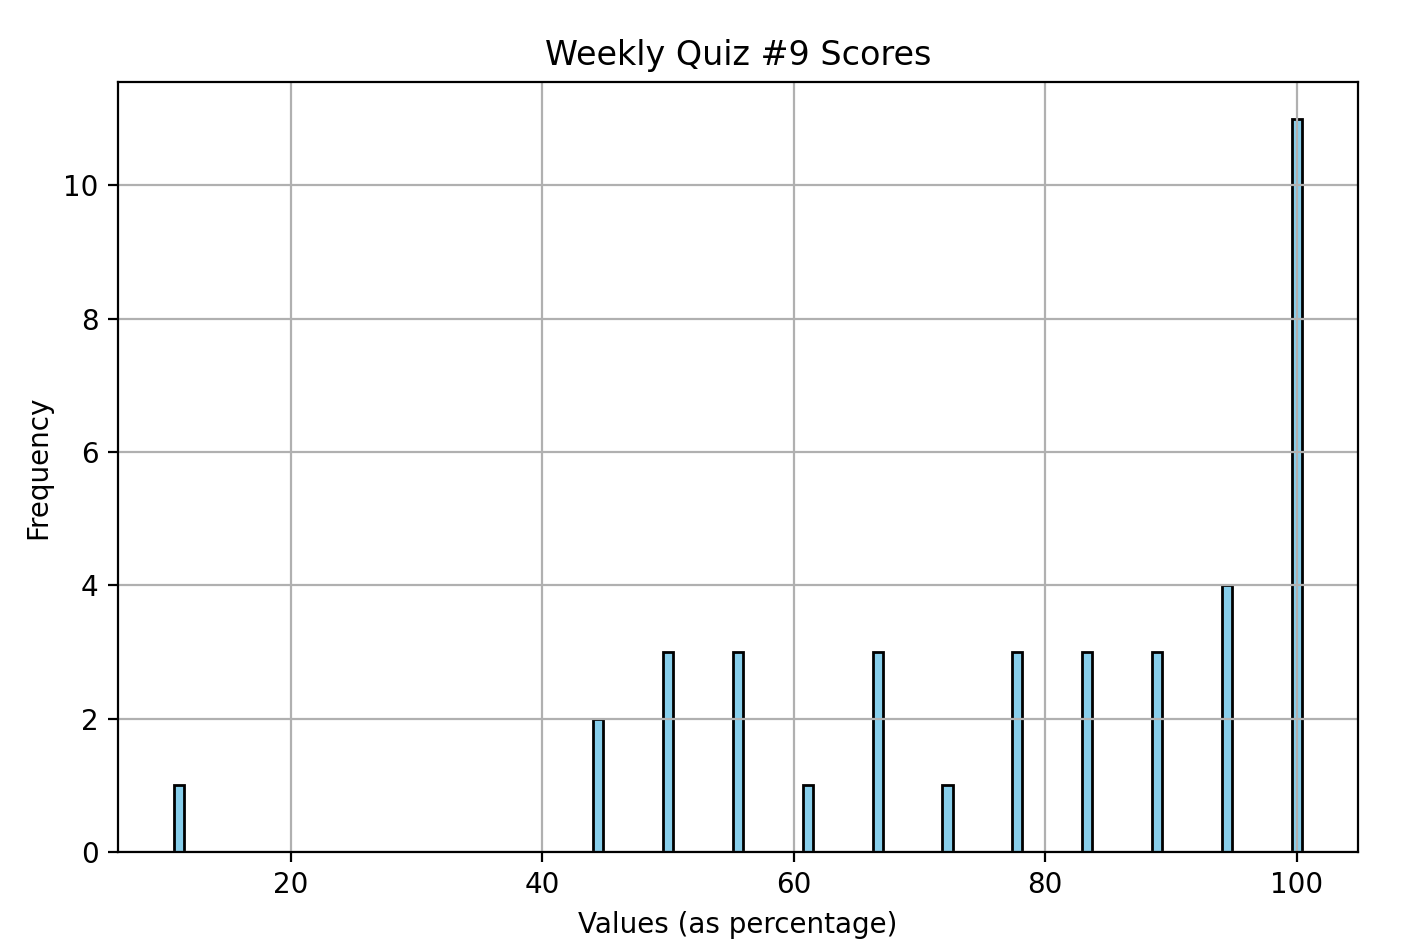
\includegraphics[width=.8\textwidth]{images/quiz_scores}
%   		 \caption{Median Score = 83\%}
%\end{figure}
%\end{frame}	


\begin{frame}{Study Guide For Quiz \#10}
\footnotesize 

\colorbox{yellow!20}{\textbf{Group exercises.}} Know how to solve the group exercises from the course meetings on Intro to Probability Part 2 (10/29), Conditional Probability and Independence (10/31), and Random Variables (11/3).


\vfill 

\colorbox{red!20}{\textbf{Readings.}}   Scheinerman Sec. 31 (Events)
\vspace{-.2cm}
\begin{itemize}
\item Know the definition of an event and how to find its probability, as given in Def 31.1 and applied in Examples 31.2-31.6. 
\item Understand how to apply the basic properties of probability, which are given in Props 31.7-31.8. 
\end{itemize}

Scheinerman Sec. 32 (Condl. Prob. and Independence)
\vspace{-.2cm}
\begin{itemize}
\item Know the definition of conditional probability (Def 32.1) and how to compute it, as in Examples 32.2-32.3.
\item Know the definition of independence (Def 32.5) and its alternate characterizations (Prop 32.4), and be able to use these to determine if events are independent.
\end{itemize}

Scheinerman Sec. 33 (Random variables)
\vspace{-.2cm}
\begin{itemize}
\item Know the definition of a random variable (Def 33.1), as applied in Examples 33.2-33.4.
\item Know how to determine whether two random variables are independent (see Def 33.6, as well as the preceding discussion).
\end{itemize}

\end{frame}



\begin{frame}[standout]
Mini-lecture: \\ 
Conditional Probability and Independence \\
(see other slide deck)
\end{frame}






\begin{frame}[standout]
Mini-lecture: Random variables
\end{frame}







\begin{frame}

\begin{myredbox}[title=\text{Practice Reading Quiz (Random Variables)}]


\begin{enumerate}
	\item Let $(S,P)$ be a probability space. What is the name for a function defined on $S$?
	\item Let $(S,P)$ be the probability space formed by rolling a pair of die.   Let $X$ be a random variable defined on this space as the sum of the values of the two dice. 
	\begin{enumerate}
	\item[a.] (True/false)  $P(X=8) = P(\set{s \in S : X(s) = 8})$.
	\item[b.] (True/false)  $P(X=8) = P(\set{(2,6), (3,5), (4,4), (5,3), (6,2)})$.
	\item[c.] (True/false)  $P(X=8) = \frac{5}{36}$.
	\item[d.] (True/false)
		$P(X \geq 8) = P(\set{s \in S : X(s) \geq 8})$.
	\end{enumerate}
\end{enumerate}
\end{myredbox}
\end{frame}


\begin{frame}{Random Variables}
\small 

\colorbox{green!30}{\textbf{Key concept.}} A \textbf{random variable} is a function on the sample space of a probability space.

\vfill 

\colorbox{blue!30}{\textbf{Example.}} Suppose we flip four coins.  The sample space consists of 16 outcomes (see below).  \onslide<2->{\alert{Which outcomes have exactly two heads?}}  \onslide<3->{We could define a random variable (function) $X$ with $X(s)=1$ (\green{green}) whenever exactly two of the coins are heads, and $X(s)=0$ (\red{red}) otherwise.}

\vfill
\centering
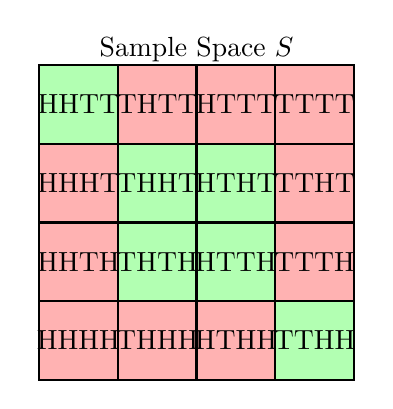
\begin{tikzpicture}
\node at (2, 4.2) {Sample Space \( S \)};
\foreach \x/\y/\outcome/\col in {
  0/0/HHHH/red,   1/0/THHH/red,   2/0/HTHH/red,   3/0/TTHH/green,
  0/1/HHTH/red,   1/1/THTH/green, 2/1/HTTH/green, 3/1/TTTH/red,
  0/2/HHHT/red,   1/2/THHT/green, 2/2/HTHT/green, 3/2/TTHT/red,
  0/3/HHTT/green, 1/3/THTT/red,   2/3/HTTT/red,   3/3/TTTT/red} {
  \only<3->{\fill[\col, opacity=0.3] (\x,\y) rectangle (\x+1,\y+1);}
  \draw[thick] (\x,\y) rectangle (\x+1,\y+1);
  \node at (\x+0.5,\y+0.5) {\outcome};
}
\end{tikzpicture}

\vfill 

\onslide<4->{\alert{What is the probability that X=1?}} \onslide<5->{$\frac{6}{16}$.}  \onslide<6->{\alert{Why?}}  \onslide<7->{Equally likely probability formula.}  
\end{frame}

\begin{frame}{Random Variables}
\begin{columns}[T,onlytextwidth]
\begin{column}{0.40\textwidth}
\centering
\textbf{Sample Space ($S$)} \\[6pt]
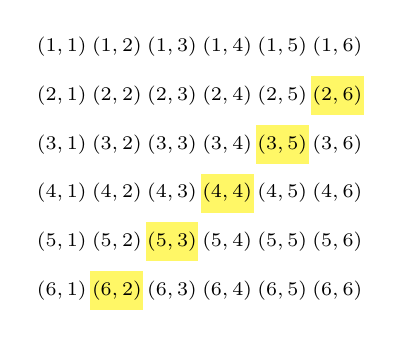
\begin{tikzpicture}[x=0.7cm, y=0.62cm]
  \foreach \a in {1,...,6} {
    \foreach \b in {1,...,6} {
      \pgfmathtruncatemacro{\total}{\a+\b}
      \ifnum\total=8
        \only<7->{\fill[yellow!60] (\b-0.48, -\a-0.4) rectangle (\b+0.48, -\a+0.4);}
      \fi
      \node[font=\scriptsize] at (\b, -\a) {$(\a,\b)$};
    }
  }
\end{tikzpicture}

\vspace{8pt}
\onslide<2->{$P(s) = \frac{1}{36}$ for all $s \in S$.}
\end{column}
\begin{column}{0.56\textwidth}
\small
\onslide<3->{Let $s = (d_1, d_2)$.}
\onslide<4->{Then $X(s) = d_1 + d_2$ is the sum of the two dice.}

\vspace{8pt}
\onslide<5->{The event that the sum is an 8 can be written $\set{X(s)=8}$, or more precisely $\set{s \in S : X(s) = 8}$.}

\vspace{8pt}
\onslide<6->{Therefore, \\[3pt]
{\footnotesize $\set{X(s)=8} = \alt<7->{\set{(2,6), (3,5), (4,4), (5,3), (6,2)}}{\;???}$\par}}

\vspace{8pt}

\onslide<8->{By the equally likely probability formula,
\[ P(X=8) = \frac{|\set{X=8}|}{|S|} = \frac{5}{36}. \]}
\end{column}
\end{columns}
\end{frame}



\begin{frame}{Solution to practice reading quiz}
\begin{myredbox}[title=\text{Practice Reading Quiz (Random Variables)}]


\begin{enumerate}
	\item Let $(S,P)$ be a probability space. What is the name for a function defined on $S$?
	\item Let $(S,P)$ be the probability space formed by rolling a pair of die.   Let $X$ be a random variable defined on this space as the sum of the values of the two dice. 
	\begin{enumerate}
	\item[a.] (True/false)  $P(X=8) = P(\set{s \in S : X(s) = 8})$.
	\item[b.] (True/false)  $P(X=8) = P(\set{(2,6), (3,5), (4,4), (5,3), (6,2)})$.
	\item[c.] (True/false)  $P(X=8) = \frac{5}{36}$.
	\item[d.] (True/false)
		$P(X \geq 8) = P(\set{s \in S : X(s) \geq 8})$.
	\end{enumerate}
\end{enumerate}
\end{myredbox}
	
\vfill 
\pause 
\begin{enumerate}
	\item Random variable. \pause 
	\item a) True \pause b) True \pause c) True \pause d) True.
\end{enumerate}
\end{frame}
%
%\begin{frame}{Binomial Random Variables}
%
%\begin{myredbox}[title=\text{Problem (Quality Control in Manufacturing)}]
%
%\begin{minipage}{.8\textwidth}
%A factory produces \textbf{LED bulbs}, and 1\% of them are defective. A random sample of 20 bulbs is shipped to a customer.
%\begin{enumerate}
%	\item  What is the probability that \textbf{exactly 0} of the 20 bulbs are defective?  
%	\item What is the probability that \textbf{no more than 1} bulb is defective? 
%\end{enumerate}
%  
%\end{minipage} % 
%\hfill 
%\begin{minipage}{.18\textwidth}
%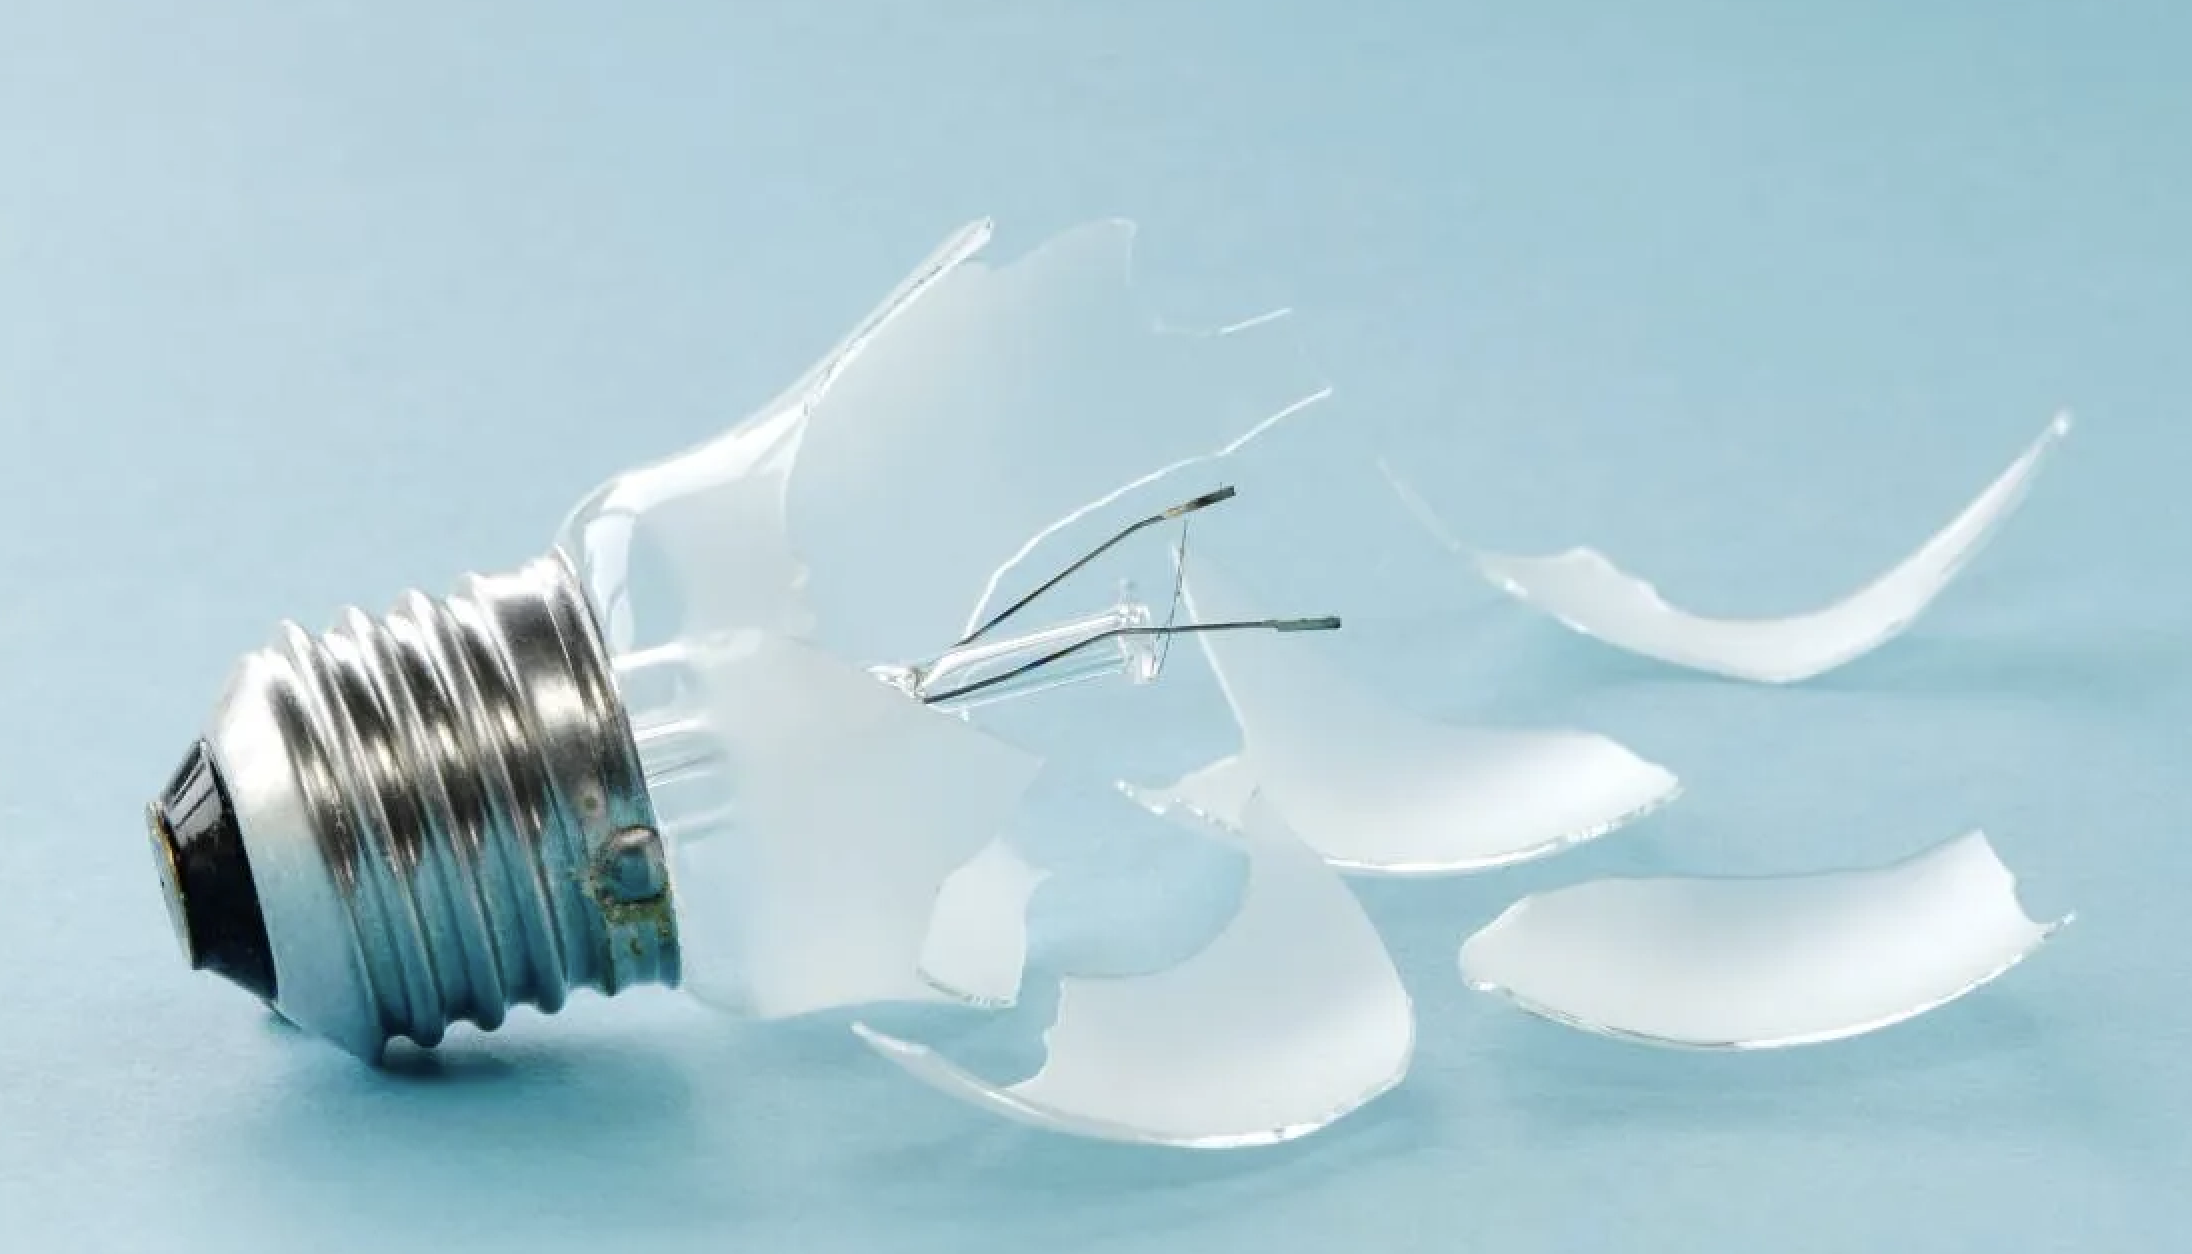
\includegraphics[width=\textwidth]{images/broken_bulb}  
%\end{minipage} % 
% 
%
%
%\end{myredbox}
%
%\vfill \vfill 
%
%\begin{mygreenbox}[title=\text{Tool: Binomial Random Variables}]
%
%A binomial random variable $X$ gives the number of successes in a sequence of $n$ independent experiments, each asking a yes–no question, where success occurs with probability $p$.  
%
%\[ P(X=x) = \binom{n}{x} p^x (1-p)^{n-x} \]
%\end{mygreenbox}
%\end{frame}



%
%\begin{frame}
%
%
%\vfill 
%\begin{myyellowbox}[title=Solution]
%Let:  
%\begin{itemize}
%\item $ n = 20$ $\rightarrow$ total bulbs tested. 
%\item $ p = 0.01$ $\rightarrow$ probability of a bulb being defective.
%\item   $X$ 	$\rightarrow$ the number of defective bulbs, which follows a \textbf{binomial distribution}
%\end{itemize}
%
%\begin{enumerate}
%	\item The probability that \textbf{exactly 0} of the 20 bulbs are defective is
%	\[P(X = 0) = \binom{20}{0} (0.01)^0 (0.99)^{20} = 0.8179\]
%	\item The probability that \textbf{no more than 1} bulb is defective is
%	\begin{align*}
%	P(X \leq 1) & = P(X = 0) + P(X = 1) \\
%	&= \binom{20}{0} (0.01)^0 (0.99)^{20} + \binom{20}{1} (0.01)^1 (0.99)^{19} \\
%	& = 0.8179 + 0.1652 = 0.9831
%	\end{align*}
%
%\end{enumerate}
%\end{myyellowbox}
%	
%\end{frame}



\begin{frame}{Binomial Random Variables}
\small

\begin{myredbox}[title=\text{Problem (False Alarms in A/B Testing)}]
You run 20 A/B tests of website changes that actually do nothing.  Each test independently has a 5\% chance of a \textbf{false alarm} (wrongly reporting that the change worked).
\begin{enumerate}
	\item What is the probability of \textbf{exactly 0} false alarms?
	\item What is the probability of \textbf{no more than 1} false alarm?
\end{enumerate}
\end{myredbox}

\vfill

\onslide<2->{\colorbox{yellow!30}{\textbf{Poll.}} Before calculating anything, take a guess at each probability.}

\vfill

\onslide<3->
\begin{mygreenbox}[title=\text{Tool: Binomial Random Variables}]
\footnotesize
A binomial random variable $X$ gives the number of successes in a sequence of $n$ independent experiments, each asking a yes--no question, where success occurs with the same probability $p$.

\[ P(X=x) = \binom{n}{x} p^x (1-p)^{n-x} \]
\end{mygreenbox}
\end{frame}


\begin{frame}
\footnotesize

\vfill 
\begin{myyellowbox}[title=Solution]
Let:  
\begin{itemize}
\item $ n = 20$ $\rightarrow$ total tests run. 
\item $ p = 0.05$ $\rightarrow$ probability of a test giving a false alarm.
\item   $X$ 	$\rightarrow$ the number of false alarms, which follows a \textbf{binomial distribution}
\end{itemize}

\begin{enumerate}
	\item The probability of \textbf{exactly 0} false alarms is
	\[P(X = 0) = \binom{20}{0} (0.05)^0 (0.95)^{20} = 0.3585\]
	\item The probability of \textbf{no more than 1} false alarm is
	\begin{align*}
	P(X \leq 1) & = P(X = 0) + P(X = 1) \\
	&= \binom{20}{0} (0.05)^0 (0.95)^{20} + \binom{20}{1} (0.05)^1 (0.95)^{19} \\
	& = 0.3585 + 0.3774 = 0.7358
	\end{align*}

\end{enumerate}
\end{myyellowbox}
	
\end{frame}



\begin{frame}{The binomial distribution: when it fits}
\begin{columns}[T,onlytextwidth]
\begin{column}{0.48\textwidth}
\onslide<1->{
\centering
\textbf{Larry Bird: pairs of free throws} \\
{\footnotesize 338 pairs, 1980--82} \\[4pt]
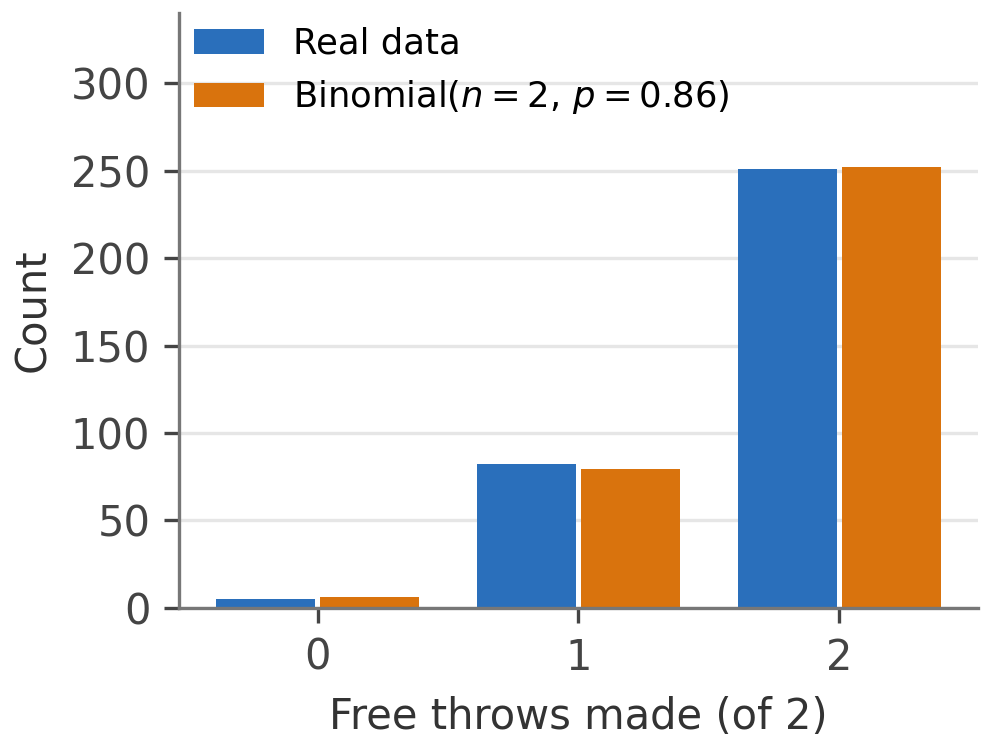
\includegraphics[width=\textwidth]{images/binomial_fit/bird}
}
\end{column}
\begin{column}{0.48\textwidth}
\onslide<2->{
\centering
\textbf{Ichiro: games with 4 at-bats} \\
{\footnotesize 931 games, 2001--12} \\[4pt]
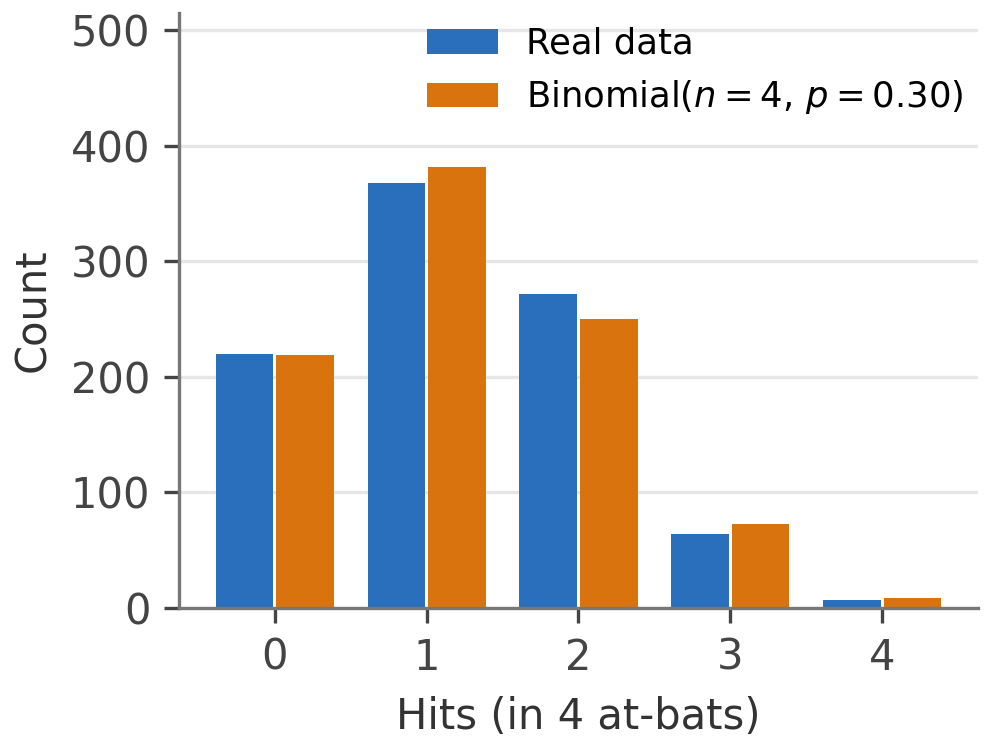
\includegraphics[width=\textwidth]{images/binomial_fit/ichiro}
}
\end{column}
\end{columns}
\end{frame}


\begin{frame}{The binomial distribution: when it doesn't fit}
\centering
\small Team wins in a season, compared to Binomial$(n, \half)$ \\[4pt]
\begin{columns}[T,onlytextwidth]
\begin{column}{0.32\textwidth}
\onslide<1->{
\centering
\textbf{NBA} {\footnotesize (2005--15)} \\[2pt]
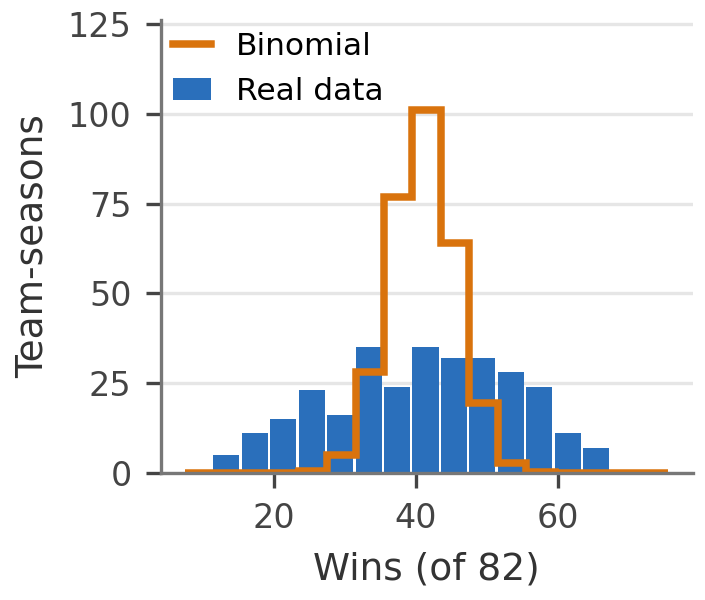
\includegraphics[width=\textwidth]{images/binomial_fit/nba_wins}
}
\end{column}
\begin{column}{0.32\textwidth}
\onslide<2->{
\centering
\textbf{NFL} {\footnotesize (2011--20)} \\[2pt]
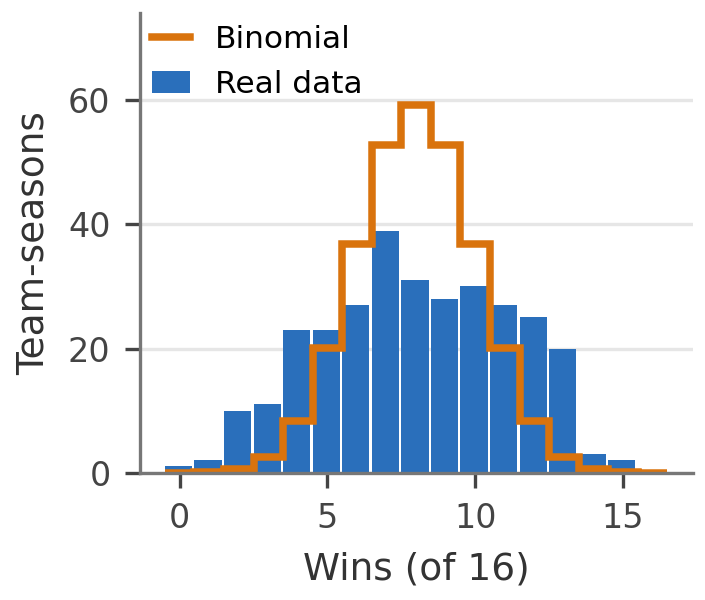
\includegraphics[width=\textwidth]{images/binomial_fit/nfl_wins}
}
\end{column}
\begin{column}{0.32\textwidth}
\onslide<3->{
\centering
\textbf{MLB} {\footnotesize (2010--19)} \\[2pt]
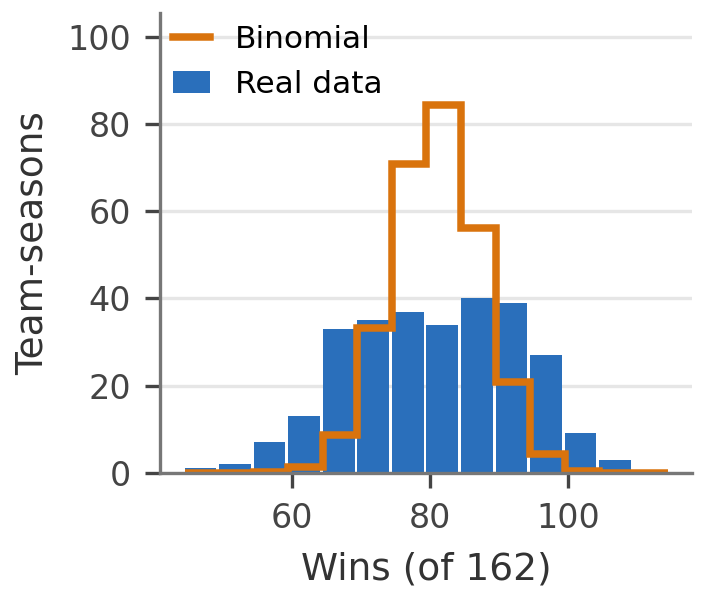
\includegraphics[width=\textwidth]{images/binomial_fit/mlb_wins}
}
\end{column}
\end{columns}
\vfill
\raggedright
\onslide<4->{\colorbox{yellow!30}{\textbf{Poll.}} Why doesn't the binomial fit?}
\vfill
\onslide<5->{\colorbox{green!30}{\textbf{Answer.}} The binomial assumes every trial has the same $p$.  But teams aren't equally good: each team has its own $p$, so win totals are far more spread out.}
\vfill
\end{frame}


\begin{frame}{The binomial distribution: when trials are dependent} 

\footnotesize

More generally, binomial distribution can fit the data poorly when trials are \alert{dependent!}

\vfill
\only<2->{
\begin{mygreenbox}[title=\text{Example 1: Election Forecasts, 2016}]
Polling errors are correlated across states: a miss in Wisconsin suggests a miss in Michigan.
\pause
\only<3->{Final odds of a Clinton win: Huffington Post 98\%; FiveThirtyEight, which modeled correlated errors, 71\%.}
\end{mygreenbox}
}

\vfill 
\only<4->{
\begin{mybluebox}[title=\text{Example 2: Mortgages and 2008 (illustrative numbers)}]
Take 1{,}000 mortgages, each with a 5\% chance of default, so we expect about 50 defaults.

\pause
\textbf{If defaults were independent (binomial):} about 99\% of the time, 33 to 69 mortgages default.  The chance of 100 or more defaults is less than \red{1 in 10 billion.}

\pause
\only<5->{\textbf{But a housing crash hits everyone at once.}  Suppose there's a 90\% chance of a healthy economy (each mortgage defaults with probability 0.03) and a 10\% chance of a crash (each defaults with probability 0.23).}

\pause
\only<6->{Each mortgage still has a 5\% chance of default: $0.9(0.03) + 0.1(0.23) = 0.05$.  But one default makes a crash, and so other defaults, more likely.}

\pause
\only<7->{Now the chance of 100 or more defaults is about \textbf{\textcolor{red!70!black}{1 in 10}}.}
\end{mybluebox}
}

\end{frame}


\begin{frame}[standout]
Group exercises
\end{frame}

\begin{frame}{Random group assignments}
%%% TABLE 1: by last name
\begin{columns}
\begin{column}{0.33\textwidth}
Ashley, Isabelle: 10 \\ 
Bailey, Tanna: 12 \\ 
Blaisdell, Olyver: 6 \\ 
Brown, Ashton: 4 \\ 
Cardenas, Dominic: 10 \\ 
Cutler, George: 2 \\ 
Fabik, Roland: 11 \\ 
Fellows, Audrey: 6 \\ 
Fitzgerald, Ryan: 7 \\ 
Fuller, Ryan: 10 \\ 
Griffen, Clara: 7 \\ 
Grutsch, Tanner: 3 \\\end{column}
\begin{column}{0.33\textwidth}
Hager, Nathan: 9 \\ 
Horner, Jayden: 5 \\ 
Johnson, Jaret: 6 \\ 
Kintzel, Samantha: 5 \\ 
Lameres, Alexis: 8 \\ 
Lee, Holden: 1 \\ 
Mayala, Reece: 11 \\ 
McLean, Connor: 9 \\ 
Mcbride, Daniel: 4 \\ 
Miller, Maverick: 2 \\ 
Moss, Emily: 9 \\ 
Mousseau, Matthew: 7 \\\end{column}
\begin{column}{0.33\textwidth}
Neuman, Evan: 3 \\ 
Putnam, John: 8 \\ 
Ramos, Vydel: 8 \\ 
Rathbun, Jedidiah: 2 \\ 
Roberts, Matthew: 12 \\ 
Roller, Nathan: 4 \\ 
Ryan, Otis: 1 \\ 
Shevtsov, Timothy: 12 \\ 
Stensland, Emma: 11 \\ 
Thiessen, Logan: 3 \\ 
Thompson, Jaiden: 1 \\ 
Vath, Ethan: 5 \\\end{column}
\end{columns}
\end{frame}


\begin{frame}{Group exercises}

\begin{enumerate}
	\item \footnotesize A fair coin is flipped three times. This is modeled by a probability space $(S,P)$ where $S$ contains the eight lists from $(H,H,H)$ to $(T,T,T)$, all with probability $\frac{1}{8}$.  Let $X$ denote the number of times we see TAILS.
	\begin{itemize}  \scriptsize  
	\item[a.] Write $X$ explicitly as a function defined on $S$.
	\item[b.] Write the event \enquote{X is odd} as a set.
	\item[c.] Calculate $P(\text{X is odd})$.
	%\item[d.] Let $Y$ denote the number of times we see HEADS.  Are $X$ and $Y$ independent?  Provide the intuition, and then a mathematical argument.
	\end{itemize}
	\item \footnotesize For each situation below, determine whether $X$ and $Y$ are independent. First provide the intuition, and then provide a mathematical argument. 
	\begin{itemize}  \scriptsize 
	\item[a.] A fair coin is flipped three times. Let $X$ be the number of heads and $Y$ be the number of tails. 
	\item[b.] A card is drawn at random from a standard deck of 52 cards. Let $X$ be the rank of the card (from 2 to ace) and $Y$ be the suit of the card.
	\item[c.] Two cards are drawn at random (without replacement) from a standard deck of 52 cards. Let $X$ be the rank of the first card and $Y$ be the rank of the second card.
	\end{itemize} 
	\item \footnotesize In a family with four children, which combination is more likely: (a) Two boys and two girls, or (b) Three of one and one of the other?
	\item \footnotesize
	A basketball player has a 75\% chance of making a free throw. During a game, the player takes 10 free throws. Model the number of free throws made as a binomial random variable. (a) What is the probability that the player makes exactly 8 free throws? (b) What is the probability that the player makes at least 7 free throws?
\end{enumerate}

\end{frame}

\begin{frame}{Solution to group exercise \#1}

\textbf{Problem.} A fair coin is flipped three times. This is modeled by a probability space $(S,P)$ where $S$ contains the eight lists from $(H,H,H)$ to $(T,T,T)$, all with probability $\frac{1}{8}$.  Let $X$ denote the number of times we see TAILS.
	\begin{itemize} \footnotesize 
	\item[a.] Write $X$ explicitly as a function defined on $S$.
	\item[b.] Write the event \enquote{X is odd} as a set.
	\item[c.] Calculate $P(\text{X is odd})$.
	\end{itemize}
\vfill 

\textbf{Solution.} 
	\begin{itemize} \small
	\item[a.]  The function $X: S \to \mathbb{N}$ is given by
	\[\begin{array}{r@{}lcr@{}l}
	X(HHH) &= 0 &\qquad & X(THH) &=1 \\
	X(HHT) &= 1 &\qquad & X(THT) &=2 \\
	X(HTH) &= 1 &\qquad & X(TTH) &=2 \\
	X(HTT) &= 2 &\qquad & X(TTT) &=3 \\
	\end{array}\]
	\item[b.] Let $A$ be the event \enquote{X is odd}.  Then $A=\set{HHT, HTH, THH, TTT}.$
	\item[c.] By the equally likely probability formula,
	\[ P(A) = \frac{|A|}{|S|}  = \frac{4}{8}. \]
	\end{itemize}
\vfill 
\end{frame}




\begin{frame}{Solution to group exercise \#2a}
\footnotesize 
\textbf{Problem.}  A fair coin is flipped three times. Let $X$ be the number of heads and $Y$ be the number of tails. Determine whether $X$ and $Y$ independent. First provide the intuition, and then provide a mathematical argument.  
\vfill 
\vspace{-.2cm}
\textbf{Solution.}
\vspace{-.2cm}
\begin{itemize}
\item \textit{Intuition.} If $X$ is the number of heads, then we \alert{know} the number of tails $Y$ \alert{exactly} (since $Y=3-X$).  So these random variables can't be independent. In fact, they are as dependent as two random variables can possibly be, since they are deterministically related.
\vfill 
\item \textit{Mathematical argument.} By Def 33.6 in Scheinerman, $X$ and $Y$ are independent if for all $x,y$

\[P(X=x \text{ and } Y=y) = P(X=x) \, P(Y=y). \]
By the above, if $x=0$, then we know $y=3$.  So let's consider $x=0$ and $y \neq 3$. In particular, let's assume $x=0$ and $y=0$.  Then 
\[ P(X=0 \text{ and } Y=0) = 0 \]
(since it's impossible for 3 coin tosses to give 0 heads and 0 tails).  However, by the equally likely probability formula,
\[P(X=0) = \frac{1}{8} \qquad \text{and} \qquad  P(Y=0) = \frac{1}{8}.\]
Hence, we have found values $x$ and $y$ such that
\[P(X=x \text{ and } Y=y) \neq P(X=x) \, P(Y=y). \]
Hence, $X$ and $Y$ are not independent.

\end{itemize}

\end{frame}


\begin{frame}{Solution to group exercise \#2b}
\small
\textbf{Problem.} A card is drawn at random from a standard deck of 52 cards. Let $X$ be the rank of the card (from 2 to ace) and $Y$ be the suit of the card. Determine whether $X$ and $Y$ independent. First provide the intuition, and then provide a mathematical argument.  
\vfill 
\vspace{-.2cm}
\textbf{Solution.}
\vspace{-.2cm}
\begin{itemize}
\item \textit{Intuition.} These random variables should be independent because knowing the suit of the card doesn't provide any information about the rank.  For instance, knowing your card is a $\heartsuit$ doesn't change the probability that it is a King.
\vfill 
\item \textit{Mathematical argument.} By Def 33.6 in Scheinerman, $X$ and $Y$ are independent if for all $x,y$
%
\begin{align}
P(X=x \text{ and } Y=y) = P(X=x) \, P(Y=y).
\label{eqn:def_independence}
\end{align}
%
Let $x$ be any value in the set $\set{2,3,4,5,6,7,8,9,10,J,Q,K,A}$.  Let $y$ be any value in $\set{\heartsuit, \diamondsuit, \spadesuit, \clubsuit}$. Then $P(X=x) = \frac{1}{13}$ and $P(Y=y) = \frac{1}{4}$.   Moreover, $P(X=x \land Y=y) = \frac{1}{52}.$  Thus, \Eqref{eqn:def_independence} is satisfied (since $\frac{1}{52} = 	\frac{1}{13} \times \frac{1}{4}$).   Hence, $X$ and $Y$ are independent random variables.
\end{itemize}

\end{frame}


\begin{frame}{Solution to group exercise \#2c}
\small 
\textbf{Problem.} Two cards are drawn at random (without replacement) from a standard deck of 52 cards. Let $X$ be the rank of the first card and $Y$ be the rank of the second card. Determine whether $X$ and $Y$ independent. First provide the intuition, and then provide a mathematical argument.  
\vfill 
\vspace{-.2cm}
\textbf{Solution.}
\vspace{-.2cm}
\begin{itemize}
\item \textit{Intuition.} These random variables should be dependent because knowing the rank of the first card provides information about the probabilities of getting various ranks for the second card.  For instance, if your first card is a king, then there is a lower probability you'll get a king on the second card (since there's one fewer king in the deck).
\vfill 
\item \textit{Mathematical argument.}  By the equally likely probability formula,
\[P(X=\texttt{King}) = \frac{4}{52} \qquad \text{and} \qquad  P(Y=\texttt{King}) = \frac{4}{52} .\]
On the other hand, we have
\[ P(X=\texttt{King} \land  Y=\texttt{King}) = \frac{4}{52} \times \frac{3}{51}\]

Hence, we have found values $x$ and $y$ such that
\[P(X=x \text{ and } Y=y) \neq P(X=x) \, P(Y=y). \]
Hence, $X$ and $Y$ are not independent.


\end{itemize}

\end{frame}




\begin{frame}{Solution to group exercise \#3}
The intuitive answer is (a) Two boys and two girls.  However, the correct answer is (b) Three of one and one of the other.
\vfill
Let $X$ be the number of boys.  We can model X as a Binomial random variable with $n=4$ and $p=\frac{1}{2}$.
\vfill 
Then the probability of the event in (a) is
\[P(X=2) = \binom{4}{2} \bigg(\half\bigg)^2 \bigg(\half\bigg)^2 = 6 \cdot \bigg(\half\bigg)^4 = \frac{6}{16}.\]

The probability of the event in (b) is $P(X=1)+P(X=3)$, where
\[P(X=1) = \binom{4}{1} \bigg(\half\bigg)^1 \bigg(\half\bigg)^3 = 4 \cdot \bigg(\half\bigg)^4 = \frac{4}{16}.\]
and similarly $P(X=3) = \frac{4}{16}$, so $P(X=1)+P(X=3)=\frac{8}{16}=\half.$

\end{frame}

\begin{frame}{Solution to group exercise \#4}
\footnotesize 
\textbf{Problem.} 	A basketball player has a 75\% chance of making a free throw. During a game, the player takes 10 free throws. Model the number of free throws made as a binomial random variable.  (a) What is the probability that the player makes exactly 8 free throws? (b) What is the probability that the player makes at least 7 free throws?
\vfill 

\small 
\textbf{Solution.} 
Let $X$ be the number of free throws made.  By the binomial assumption, the probability that the random variable $X$ takes on the specific value $x \in \set{0,1,\hdots, 10}$ is given by
%
\begin{align*}
P(X=x) &= \binom{n}{x} p^x \, (1-p)^{n-x} = \binom{10}{x} .75^x \, (.25)^{10-x} 
\end{align*}
%
\vspace{-.2cm}
\begin{itemize}\small   
	\item[a.] By the above
	\[P(X=8) = \binom{10}{8} .75^8\, (.25)^{2} \approx 0.28 \]
	So there is an approximately 28\% chance that the player makes 8 of the 10 free throws.
	\item[b.] Using similar computations as above, we can compute
	%
	\begin{align*}
	P(X \geq 7) &= P(X=7) + P(X=8) + P(X=9) + P(X=10) \\
	& \approx 0.25 + 0.28 + 0.18 + 0.05 = 0.76.
	\end{align*}
	\end{itemize}
		
\vfill 
\end{frame}






\end{document}
